\documentclass[12pt]{extarticle}
\usepackage[T1]{fontenc}
\usepackage[utf8]{inputenc}
\usepackage[english]{babel}
\usepackage[a4paper,left=3cm,right=2.2cm,top=2.5cm,bottom=2.5cm]{geometry}
\usepackage{graphicx}
\usepackage{array}
\usepackage{longtable}
\usepackage{booktabs}
\usepackage{hyperref}
\usepackage{xcolor}
\usepackage{enumitem}
\usepackage{listings}
\usepackage{float}
\usepackage{titlesec}

\hypersetup{
    colorlinks=true,
    linkcolor=black,
    urlcolor=blue,
    pdftitle={Cyberpunk: Echoes Below - Final Documentation},
    pdfauthor={Andrii Mykhalko}
}

\titleformat{\section}{\large\bfseries}{\thesection}{0.75em}{}
\titleformat{\subsection}{\normalsize\bfseries}{\thesubsection}{0.75em}{}

\lstset{
    basicstyle=\ttfamily\small,
    breaklines=true,
    frame=single,
    columns=fullflexible,
    language=Java
}

\begin{document}

\begin{titlepage}
    \centering
    {\Large Slovak University of Technology in Bratislava\par}
    \vspace{0.5cm}
    {\Large Faculty of Informatics and Information Technologies\par}
    \vfill
    {\Large Andrii Mykhalko\par}
    \vspace{1.2cm}
    {\Huge \textbf{Cyberpunk: Echoes Below}\par}
    \vspace{0.4cm}
    {\Large Final Technical Documentation\par}
    \vspace{0.4cm}
    {\large Assignment 3 - Final Submission\par}
    \vfill
    \begin{flushright}
        Study program: B-INFO, 1st year\\
        Course: OOP\\
        Submission date: \today
    \end{flushright}
\end{titlepage}

\tableofcontents
\newpage

\section{Introduction}
Cyberpunk: Echoes Below is a Java game built as a combination of a reusable modular engine and an orchestrator turning engine into a real complete game. The final result is a top-down cyberpunk action experience in which the player explores a hostile environment, fights enemies, uses melee and ranged weapons, manages inventory, completes quests, and interacts with world mechanisms such as gates and levers.

The implementation is divided into many focused Gradle modules. Core engine functionality is separated into subsystems for entities, events, scheduling, ticking, world management, transforms, physics, graphics, AI, inventory, equipment, quests, audio, and characteristic handling. The \texttt{game} module uses these modules to assemble the final gameplay loop and user interface.

The goal of this documentation is to show how the final submission satisfies the required course conditions, summarize the technical architecture, and explain the main design decisions and implementation techniques used in the project.

\section{Project Overview}
\subsection{Gameplay Summary}
The player controls a character in a cyberpunk environment rendered with LibGDX. During gameplay the player can:
\begin{itemize}[leftmargin=1.5em]
    \item move around the map using keyboard input,
    \item fight enemies with a sword, handgun, and rifle,
    \item receive visual and audio feedback during combat,
    \item pick up, use, equip, and manage items,
    \item heal through consumables and temporary effects,
    \item complete quest objectives displayed on the HUD,
    \item interact with mechanisms that change the level state,
    \item lose the game and see a dedicated game-over interface.
\end{itemize}

\subsection{Technology Stack}
The project is implemented in Java and built with Gradle. The most important technologies used are:
\begin{itemize}[leftmargin=1.5em]
    \item \textbf{LibGDX} for the desktop application, rendering, textures, audio, and GUI components,
    \item \textbf{JUnit 5} and \textbf{Mockito} for automated testing,
    \item \textbf{JaCoCo} for code coverage measurement,
    \item \textbf{SLF4J} with \textbf{Logback} for activity logging,
    \item \textbf{JGraphT} for graph-based utility structures and pathfinding support,
    \item \textbf{Lombok} for selected annotations such as logging support.
\end{itemize}

\section{Architecture}
\subsection{Modular Structure}
The repository is organized as a multi-module Gradle project. The architecture separates interfaces from implementations and isolates responsibilities into engine subsystems. Important modules include:
\begin{itemize}[leftmargin=1.5em]
    \item \texttt{commons}: shared graph, identity, task, and workflow utilities,
    \item \texttt{system} and \texttt{system-manager}: system abstraction and registration/orchestration,
    \item \texttt{entity}, \texttt{world}, \texttt{transform}, \texttt{physics}, \texttt{graphics}: basic simulation and rendering data,
    \item \texttt{event}, \texttt{scheduler}, \texttt{tick}: communication and timed execution,
    \item \texttt{ai}, \texttt{inventory}, \texttt{equipment}, \texttt{quest}, \texttt{audio}, \texttt{characteristic}: higher-level gameplay services,
    \item \texttt{game}: concrete game logic, UI, launcher, rendering integration, combat, mechanisms, quests, and AI strategies.
\end{itemize}

\subsection{System Composition}
The main integration point is the \texttt{EchoesBelowGame} class, which initializes engine systems, registers characteristics, configures controls, creates game entities, and coordinates runtime behavior. The desktop entry point is \texttt{DesktopLauncher}, which configures the LibGDX application window and starts the game.

The architecture follows an engine-on-bottom, game-on-top layering:
\begin{itemize}[leftmargin=1.5em]
    \item low-level data and execution services provide reusable abstractions,
    \item engine subsystems expose interfaces and concrete \texttt{*Impl} implementations,
    \item the game module composes them into a finished application with cyberpunk gameplay.
\end{itemize}

\subsection{Execution Flow}
The runtime loop is based on multiple cooperating systems:
\begin{itemize}[leftmargin=1.5em]
    \item input events are captured by the input system and translated into binding events,
    \item gameplay systems react to events and modify entity state,
    \item physics and transform systems update movement and collision state,
    \item AI systems update enemy behavior,
    \item rendering and UI systems read the current state and draw the scene and overlays,
    \item quest, inventory, equipment, and mechanism systems update the player's progress and world interactions.
\end{itemize}

\section{Required Conditions}
\subsection{Object-Oriented Programming Principles}
The project was intentionally designed around OOP principles required by the assignment.

\subsubsection{Abstraction}
Abstraction is present throughout the engine through interfaces such as \texttt{AiStrategy}, \texttt{AiSystem}, \texttt{GraphicsSystem}, \texttt{AudioSystem}, \texttt{WorldSystem}, \texttt{InventorySystem}, \texttt{QuestSystem}, and \texttt{EventManager}. Each interface defines behavior independently from a specific implementation.

\begin{lstlisting}[caption={Interface-based abstraction through the AI strategy contract}]
public interface AiStrategy {
    void update(long entityId);
}
\end{lstlisting}

\subsubsection{Encapsulation}
Engine and gameplay classes hide internal state behind methods and private fields. Examples include caches and concurrent maps in rendering, AI, audio, physics, and gameplay systems. This keeps the public API focused while protecting internal data structures from accidental misuse.

\subsubsection{Inheritance and Interface Implementation}
Concrete implementations follow the interface-first design of the project. Examples include \texttt{WorldSystemImpl}, \texttt{TransformSystemImpl}, \texttt{PhysicsSystemImpl}, \texttt{GraphicsSystemImpl}, \texttt{InventorySystemImpl}, \texttt{QuestSystemImpl}, and \texttt{DefaultEventManager}. These classes provide implementation details while preserving a common contract for the rest of the engine.

\subsubsection{Polymorphism}
\textbf{Run-time polymorphism} is used in multiple ways:
\begin{itemize}[leftmargin=1.5em]
    \item AI behavior is selected through the \texttt{AiStrategy} interface and replaced with implementations such as \texttt{ChasingAiStrategy}, \texttt{MeleeAiStrategy}, and \texttt{PathfindingAiStrategy}.
    \item Rendering behavior depends on the concrete graphics type, for example \texttt{TextureGraphics}, \texttt{AnimationGraphics}, and \texttt{TiledWorldGraphics}.
    \item Systems are stored and managed through shared abstraction rather than direct hard-coded coupling.
\end{itemize}

\textbf{Compile-time polymorphism} is present through generic abstractions such as \texttt{Graph<TVertex, TEdge>}, \texttt{Task<TResult>}, \texttt{TaskDescriptor<TResult>}, \texttt{TaskRunnable<TResult>}, and related workflow classes.

\subsubsection{Overloading and Overriding}
Overloading is used, for example, in constructors such as \texttt{PathfindingAiStrategy}, which provides multiple constructor variants for different configuration needs. Overriding is used throughout the codebase in methods such as \texttt{init()}, \texttt{tick()}, \texttt{update()}, \texttt{render()}, and event listener callbacks.

\begin{lstlisting}[caption={Constructor overloading in PathfindingAiStrategy}]
public PathfindingAiStrategy(long targetEntityId, long worldId,
                             TransformSystem transformSystem,
                             PhysicsSystem physicsSystem,
                             CharacteristicSystem characteristicSystem,
                             double tileSize, int gridWidth, int gridHeight) {
    this(targetEntityId, worldId, transformSystem, physicsSystem,
         characteristicSystem, tileSize, gridWidth, gridHeight,
         AiVisibility.DEFAULT_DETECTION_RANGE);
}

public PathfindingAiStrategy(long targetEntityId, long worldId,
                             TransformSystem transformSystem,
                             PhysicsSystem physicsSystem,
                             CharacteristicSystem characteristicSystem,
                             double tileSize, int gridWidth, int gridHeight,
                             double detectionRange) {
    this.targetEntityId = targetEntityId;
    this.worldId = worldId;
    this.transformSystem = transformSystem;
    this.physicsSystem = physicsSystem;
    this.characteristicSystem = characteristicSystem;
    this.tileSize = tileSize;
    this.gridWidth = gridWidth;
    this.gridHeight = gridHeight;
    this.detectionRange = detectionRange;
}
\end{lstlisting}

\subsection{Graphical User Interface}
The project includes a functional graphical user interface built with LibGDX. It contains both in-world rendering and overlay-based UI.

The GUI consists of:
\begin{itemize}[leftmargin=1.5em]
    \item \texttt{LibGdxRenderingSystem} for world and entity rendering,
    \item \texttt{HudUI} for displaying player health and heart icons,
    \item \texttt{InventoryUI} for item display and interaction,
    \item \texttt{QuestHudUI} for active quest progress,
    \item \texttt{GameOverUI} for end-of-game feedback,
    \item \texttt{DesktopLauncher} for starting the desktop windowed application.
\end{itemize}

The interface is not purely decorative. It is directly connected to gameplay state through events, characteristics, inventory contents, equipped items, and quest progress.

\begin{figure}[H]
    \centering
    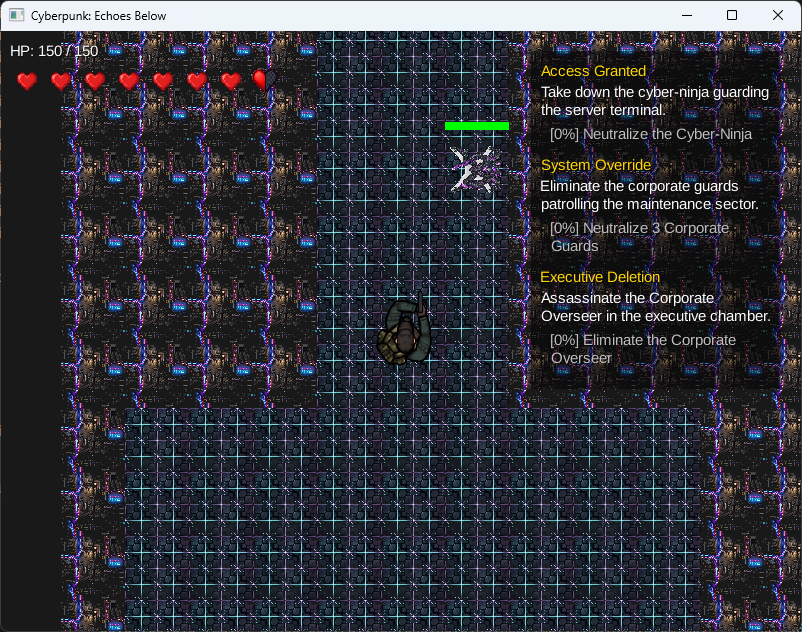
\includegraphics[width=\textwidth]{docs/placeholders/gameplay-screenshot-placeholder.png}
    \caption{Placeholder file for the gameplay screenshot. Replace this file with a real in-game screenshot.}
\end{figure}

\begin{figure}[H]
    \centering
    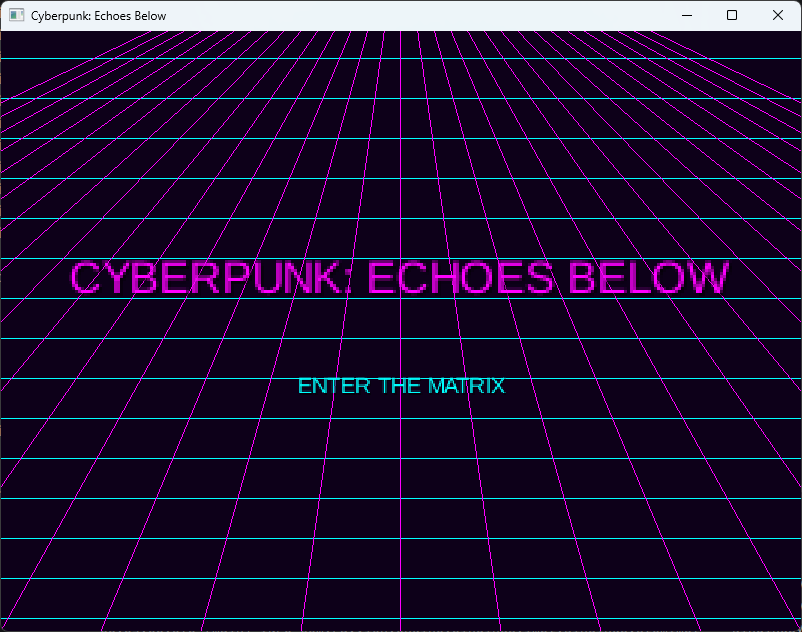
\includegraphics[width=\textwidth]{docs/placeholders/main-menu-screenshot-placeholder.png}
    \caption{Placeholder file for the main menu screenshot. Replace this file with a screenshot of the title screen or start menu.}
\end{figure}

\begin{figure}[H]
    \centering
    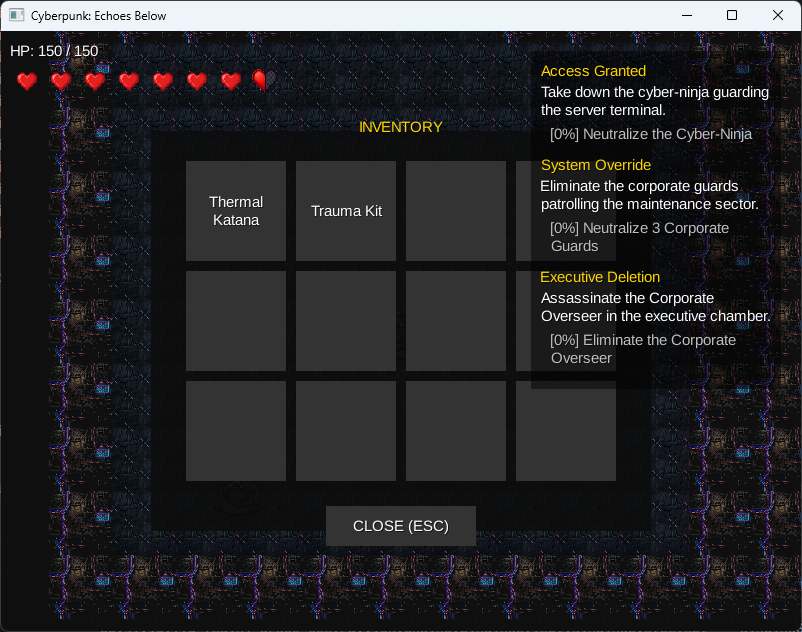
\includegraphics[width=\textwidth]{docs/placeholders/ui-screenshot-placeholder.png}
    \caption{Placeholder file for an optional UI screenshot such as the inventory, quest HUD, or game-over screen.}
\end{figure}

\subsection{Interfaces}
The project contains many meaningful interfaces and uses them as a central architectural rule. This is one of the strongest parts of the solution. Interfaces define engine services and decouple high-level game logic from implementation details. Examples include \texttt{System}, \texttt{Tickable}, \texttt{EventManager}, \texttt{SchedulerSystem}, \texttt{PhysicsSystem}, \texttt{TransformSystem}, \texttt{GraphicsSystem}, \texttt{AudioSystem}, and \texttt{AiStrategy}.

\subsection{Unit Tests and Coverage}
The project contains broad automated test coverage across engine and gameplay modules. Tests are present for common infrastructure and for concrete gameplay features such as animation state handling, input, quests, movement, combat systems, AI behavior, audio, mechanisms, inventory, physics, graphics, events, equipment, and tick execution.

JaCoCo is configured in the Gradle build across the project modules and is used for code coverage reporting. The final project meets the required unit test coverage threshold of at least 80\%.

\subsection{JavaDoc}
The codebase includes JavaDoc comments.

\section{Additional Conditions}
\subsection{Design Patterns}
\subsubsection{Strategy Pattern}
The Strategy pattern is used in the AI subsystem. The \texttt{AiStrategy} interface defines the contract for enemy behavior, while concrete strategies such as \texttt{ChasingAiStrategy}, \texttt{MeleeAiStrategy}, and \texttt{PathfindingAiStrategy} provide different movement and combat logic. The AI system can change a strategy at runtime depending on the entity and desired behavior.

This implementation is meaningful because different enemies can reuse the same AI infrastructure while exhibiting distinct behavior.





\begin{lstlisting}[caption={Strategy pattern through interchangeable AI behaviors}]
public interface AiStrategy {
    void update(long entityId);
}

public class PathfindingAiStrategy implements AiStrategy {
    @Override
    public void update(long entityId) {
        // Recalculate and follow an A* path toward the target.
    }
}
\end{lstlisting}

\subsubsection{Observer Pattern}
The Observer pattern is implemented through the event subsystem. \texttt{DefaultEventManager} allows components to register event types, publish events, and subscribe with push or pull semantics. Systems such as movement, UI, inventory, quests, and combat react to published events without being tightly coupled to the sender.

This implementation is meaningful because it reduces direct dependencies between systems and helps the engine remain modular.





\begin{lstlisting}[caption={Observer pattern through event publication and subscription}]
@Override
public <T extends Event> void publish(T event) {
    Class<? extends Event> eventClass = event.getClass();
    Set<Class<?>> assignableTypes = getAssignableTypes(eventClass);

    for (Class<?> type : assignableTypes) {
        List<Consumer<Event>> consumers = pushSubscribers.get(type);
        if (consumers != null) {
            for (Consumer<Event> consumer : consumers) {
                consumer.accept(event);
            }
        }
    }
}

@Override
public <T extends Event> void subscribe(Class<T> eventType, Consumer<T> subscriber) {
    pushSubscribers
        .computeIfAbsent(eventType, k -> new CopyOnWriteArrayList<>())
        .add((Consumer<Event>) subscriber);
}
\end{lstlisting}

\subsection{Activity Logging}
The project uses the SLF4J logging API with Logback as the runtime backend. Logging is integrated into multiple subsystems including bindings, events, game startup, AI, audio, combat, physics, tick scheduling, quests, and UI activation.

Meaningful runtime information is logged with multiple levels:
\begin{itemize}[leftmargin=1.5em]
    \item \texttt{INFO} for major state changes and important gameplay events,
    \item \texttt{DEBUG} for lower-level diagnostic information,
    \item \texttt{WARN} for suspicious but recoverable situations,
    \item \texttt{ERROR} for failures and caught exceptions,
    \item \texttt{TRACE} for very detailed runtime tracing.
\end{itemize}

\begin{lstlisting}[caption={Logging with multiple levels in the event and game systems}]
@Slf4j
public class DefaultEventManager implements EventManager {
    @Override
    public void init() {
        log.info("Initializing DefaultEventManager");
    }
}

log.debug("EchoesBelowGame: BindingEvent: {} Type: {}",
          event.parameter().name(), event.type());
log.error("Exception in event subscriber for event type: {}",
          eventClass.getName(), e);
\end{lstlisting}

\subsection{Multithreading}
Multithreading is implemented in the workflow and scheduling infrastructure. \texttt{DefaultWorkflowExecution} uses an \texttt{ExecutorService} and \texttt{CompletableFuture} to execute tasks asynchronously. \texttt{DefaultSchedulerSystem} uses a \texttt{ScheduledExecutorService} to run workflows at one-time, fixed-rate, and fixed-delay schedules.

Proper synchronization of resource access is addressed through:
\begin{itemize}[leftmargin=1.5em]
    \item \texttt{ConcurrentHashMap} and concurrent key sets,
    \item synchronized methods and synchronized blocks,
    \item controlled access to shared lists and world state,
    \item separation of task status tracking and result storage in workflow execution.
\end{itemize}

\begin{lstlisting}[caption={Executor-based multithreading in the scheduler system}]
private final ScheduledExecutorService executorService;
private final Map<ScheduledWorkflow, ScheduledFuture<?>> activeExecutions
        = new ConcurrentHashMap<>();

public DefaultSchedulerSystem(SystemDescriptor descriptor) {
    this.descriptor = descriptor;
    this.executorService = Executors.newScheduledThreadPool(
            Runtime.getRuntime().availableProcessors());
}

ScheduledFuture<?> future = switch (schedule) {
    case Schedule.OneTime(Duration delay) ->
        executorService.schedule(() -> runWorkflow(workflow),
            delay.toMillis(), TimeUnit.MILLISECONDS);
    case Schedule.FixedRate(Duration initialDelay, Duration period) ->
        executorService.scheduleAtFixedRate(() -> runWorkflow(workflow),
            initialDelay.toMillis(), period.toMillis(), TimeUnit.MILLISECONDS);
    case Schedule.FixedDelay(Duration initialDelay, Duration delay) ->
        executorService.scheduleWithFixedDelay(() -> runWorkflow(workflow),
            initialDelay.toMillis(), delay.toMillis(), TimeUnit.MILLISECONDS);
};
\end{lstlisting}

\subsection{Generics}
Generics are used meaningfully in the engine, especially in reusable infrastructure. Examples include:
\begin{itemize}[leftmargin=1.5em]
    \item \texttt{Graph<TVertex, TEdge>},
    \item \texttt{DefaultDirectedGraph<TVertex, TEdge>},
    \item \texttt{Task<TResult>},
    \item \texttt{TaskDescriptor<TResult>},
    \item \texttt{TaskRunnable<TResult>},
    \item namespaced identity abstractions.
\end{itemize}

These generic types improve type safety and allow the same infrastructure to support many different data and execution scenarios.

\begin{lstlisting}[caption={Generic task abstraction used by the workflow infrastructure}]
public record Task<TResult>(
        TaskDescriptor<TResult> descriptor,
        TaskRunnable<TResult> runnable
) { }
\end{lstlisting}

\subsection{Reflection}
The project uses a lightweight but real form of reflection in the event system. In \texttt{DefaultEventManager}, published events are inspected at runtime via \texttt{event.getClass()} to determine the concrete event type and collect assignable types for subscriber dispatch. This enables dynamic routing of events based on runtime type information instead of hard-coded direct calls.

\begin{lstlisting}[caption={Runtime type inspection used for event dispatch}]
public <T extends Event> void publish(T event) {
    Class<? extends Event> eventClass = event.getClass();
    if (!registeredEvents.contains(eventClass)) {
        throw new IllegalArgumentException(
            "Event type not registered: " + eventClass.getName());
    }

    Set<Class<?>> assignableTypes = getAssignableTypes(eventClass);
    // Dispatch to subscribers based on runtime type hierarchy.
}
\end{lstlisting}

\subsection{Lambda Expressions}
Lambda expressions are used in several meaningful parts of the project:
\begin{itemize}[leftmargin=1.5em]
    \item event subscribers reacting to gameplay and UI events,
    \item task and scheduler callbacks executed asynchronously,
    \item pathfinding heuristics in the A* implementation,
    \item map and cache initialization with \texttt{computeIfAbsent},
    \item tests that define compact behavior stubs and expectations.
\end{itemize}

\begin{lstlisting}[caption={Lambda expressions in scheduling and pathfinding}]
case Schedule.OneTime(Duration delay) ->
    executorService.schedule(() -> runWorkflow(workflow),
        delay.toMillis(), TimeUnit.MILLISECONDS);

AStarShortestPath<Node, DefaultWeightedEdge> astar =
    new AStarShortestPath<>(graph, (n1, n2) ->
        Math.sqrt(Math.pow(n1.x - n2.x, 2) + Math.pow(n1.y - n2.y, 2)));
\end{lstlisting}

\subsection{Not Claimed Features}
The following optional features are not claimed in this documentation because they are not part of the implemented final evidence used here:
\begin{itemize}[leftmargin=1.5em]
    \item custom exception classes,
    \item serialization support.
\end{itemize}

\section{Testing and Quality Assurance}
\subsection{Automated Testing}
Testing is a major part of the project. The codebase contains a large set of unit tests distributed across both engine and game modules. Examples include tests for:
\begin{itemize}[leftmargin=1.5em]
    \item graph and workflow utilities,
    \item event dispatching,
    \item system management,
    \item tick execution,
    \item physics and graphics integration,
    \item bindings, inventory, equipment, and quests,
    \item animation state management,
    \item movement and input,
    \item AI strategies,
    \item combat systems such as sword, handgun, rifle, healing, damage feedback, and death handling,
    \item audio and gameplay mechanisms.
\end{itemize}

\subsection{Coverage}
JaCoCo is configured in the Gradle build files and connected to test execution. Coverage reports are therefore part of the project workflow, and the final tested implementation satisfies the assignment requirement of at least 80\% unit test coverage.

\subsection{Documentation and Maintainability}
Maintainability is supported by:
\begin{itemize}[leftmargin=1.5em]
    \item separation of interfaces and implementations,
    \item modular Gradle structure,
    \item JavaDoc comments,
    \item logging for debugging and monitoring,
    \item unit tests for engine and gameplay logic.
\end{itemize}

\section{Commit History Note}
The project was developed continuously in the GitHub repository during the semester. One week, specifically \texttt{2026-W08}, contains only one commit.

\section{Conclusion}
The final implementation includes a graphical user interface, broad unit testing, strong use of interfaces, documented source code, and multiple additional technical features such as design patterns, logging, multithreading, generics, reflection, and lambda expressions.

From an OOP perspective, the project demonstrates abstraction, encapsulation, inheritance, polymorphism, overloading, and overriding in a meaningful and practical way. From a software engineering perspective, it emphasizes modularity, reusability, maintainability, and automated verification. The result is not only a game, but also a structured example of object-oriented system design applied to an interactive software product.

\end{document}
